% Options for packages loaded elsewhere
\PassOptionsToPackage{unicode}{hyperref}
\PassOptionsToPackage{hyphens}{url}
%
\documentclass[
]{article}
\usepackage{amsmath,amssymb}
\usepackage{lmodern}
\usepackage{iftex}
\ifPDFTeX
  \usepackage[T1]{fontenc}
  \usepackage[utf8]{inputenc}
  \usepackage{textcomp} % provide euro and other symbols
\else % if luatex or xetex
  \usepackage{unicode-math}
  \defaultfontfeatures{Scale=MatchLowercase}
  \defaultfontfeatures[\rmfamily]{Ligatures=TeX,Scale=1}
\fi
% Use upquote if available, for straight quotes in verbatim environments
\IfFileExists{upquote.sty}{\usepackage{upquote}}{}
\IfFileExists{microtype.sty}{% use microtype if available
  \usepackage[]{microtype}
  \UseMicrotypeSet[protrusion]{basicmath} % disable protrusion for tt fonts
}{}
\makeatletter
\@ifundefined{KOMAClassName}{% if non-KOMA class
  \IfFileExists{parskip.sty}{%
    \usepackage{parskip}
  }{% else
    \setlength{\parindent}{0pt}
    \setlength{\parskip}{6pt plus 2pt minus 1pt}}
}{% if KOMA class
  \KOMAoptions{parskip=half}}
\makeatother
\usepackage{xcolor}
\IfFileExists{xurl.sty}{\usepackage{xurl}}{} % add URL line breaks if available
\IfFileExists{bookmark.sty}{\usepackage{bookmark}}{\usepackage{hyperref}}
\hypersetup{
  pdftitle={Bootstraping\_Regrission},
  hidelinks,
  pdfcreator={LaTeX via pandoc}}
\urlstyle{same} % disable monospaced font for URLs
\usepackage[margin=1in]{geometry}
\usepackage{color}
\usepackage{fancyvrb}
\newcommand{\VerbBar}{|}
\newcommand{\VERB}{\Verb[commandchars=\\\{\}]}
\DefineVerbatimEnvironment{Highlighting}{Verbatim}{commandchars=\\\{\}}
% Add ',fontsize=\small' for more characters per line
\usepackage{framed}
\definecolor{shadecolor}{RGB}{248,248,248}
\newenvironment{Shaded}{\begin{snugshade}}{\end{snugshade}}
\newcommand{\AlertTok}[1]{\textcolor[rgb]{0.94,0.16,0.16}{#1}}
\newcommand{\AnnotationTok}[1]{\textcolor[rgb]{0.56,0.35,0.01}{\textbf{\textit{#1}}}}
\newcommand{\AttributeTok}[1]{\textcolor[rgb]{0.77,0.63,0.00}{#1}}
\newcommand{\BaseNTok}[1]{\textcolor[rgb]{0.00,0.00,0.81}{#1}}
\newcommand{\BuiltInTok}[1]{#1}
\newcommand{\CharTok}[1]{\textcolor[rgb]{0.31,0.60,0.02}{#1}}
\newcommand{\CommentTok}[1]{\textcolor[rgb]{0.56,0.35,0.01}{\textit{#1}}}
\newcommand{\CommentVarTok}[1]{\textcolor[rgb]{0.56,0.35,0.01}{\textbf{\textit{#1}}}}
\newcommand{\ConstantTok}[1]{\textcolor[rgb]{0.00,0.00,0.00}{#1}}
\newcommand{\ControlFlowTok}[1]{\textcolor[rgb]{0.13,0.29,0.53}{\textbf{#1}}}
\newcommand{\DataTypeTok}[1]{\textcolor[rgb]{0.13,0.29,0.53}{#1}}
\newcommand{\DecValTok}[1]{\textcolor[rgb]{0.00,0.00,0.81}{#1}}
\newcommand{\DocumentationTok}[1]{\textcolor[rgb]{0.56,0.35,0.01}{\textbf{\textit{#1}}}}
\newcommand{\ErrorTok}[1]{\textcolor[rgb]{0.64,0.00,0.00}{\textbf{#1}}}
\newcommand{\ExtensionTok}[1]{#1}
\newcommand{\FloatTok}[1]{\textcolor[rgb]{0.00,0.00,0.81}{#1}}
\newcommand{\FunctionTok}[1]{\textcolor[rgb]{0.00,0.00,0.00}{#1}}
\newcommand{\ImportTok}[1]{#1}
\newcommand{\InformationTok}[1]{\textcolor[rgb]{0.56,0.35,0.01}{\textbf{\textit{#1}}}}
\newcommand{\KeywordTok}[1]{\textcolor[rgb]{0.13,0.29,0.53}{\textbf{#1}}}
\newcommand{\NormalTok}[1]{#1}
\newcommand{\OperatorTok}[1]{\textcolor[rgb]{0.81,0.36,0.00}{\textbf{#1}}}
\newcommand{\OtherTok}[1]{\textcolor[rgb]{0.56,0.35,0.01}{#1}}
\newcommand{\PreprocessorTok}[1]{\textcolor[rgb]{0.56,0.35,0.01}{\textit{#1}}}
\newcommand{\RegionMarkerTok}[1]{#1}
\newcommand{\SpecialCharTok}[1]{\textcolor[rgb]{0.00,0.00,0.00}{#1}}
\newcommand{\SpecialStringTok}[1]{\textcolor[rgb]{0.31,0.60,0.02}{#1}}
\newcommand{\StringTok}[1]{\textcolor[rgb]{0.31,0.60,0.02}{#1}}
\newcommand{\VariableTok}[1]{\textcolor[rgb]{0.00,0.00,0.00}{#1}}
\newcommand{\VerbatimStringTok}[1]{\textcolor[rgb]{0.31,0.60,0.02}{#1}}
\newcommand{\WarningTok}[1]{\textcolor[rgb]{0.56,0.35,0.01}{\textbf{\textit{#1}}}}
\usepackage{graphicx}
\makeatletter
\def\maxwidth{\ifdim\Gin@nat@width>\linewidth\linewidth\else\Gin@nat@width\fi}
\def\maxheight{\ifdim\Gin@nat@height>\textheight\textheight\else\Gin@nat@height\fi}
\makeatother
% Scale images if necessary, so that they will not overflow the page
% margins by default, and it is still possible to overwrite the defaults
% using explicit options in \includegraphics[width, height, ...]{}
\setkeys{Gin}{width=\maxwidth,height=\maxheight,keepaspectratio}
% Set default figure placement to htbp
\makeatletter
\def\fps@figure{htbp}
\makeatother
\setlength{\emergencystretch}{3em} % prevent overfull lines
\providecommand{\tightlist}{%
  \setlength{\itemsep}{0pt}\setlength{\parskip}{0pt}}
\setcounter{secnumdepth}{-\maxdimen} % remove section numbering
\ifLuaTeX
  \usepackage{selnolig}  % disable illegal ligatures
\fi

\title{Bootstraping\_Regrission}
\author{}
\date{\vspace{-2.5em}}

\begin{document}
\maketitle

\hypertarget{a-bootstrapping}{%
\section{a) Bootstrapping}\label{a-bootstrapping}}

\hypertarget{section}{%
\subsection{1)}\label{section}}

\begin{Shaded}
\begin{Highlighting}[]
\NormalTok{data }\OtherTok{=}\NormalTok{ airquality}\SpecialCharTok{$}\NormalTok{Solar.R}
\NormalTok{boot\_sample }\OtherTok{=} \FunctionTok{as.list}\NormalTok{(}\FunctionTok{as.data.frame}\NormalTok{(}\FunctionTok{replicate}\NormalTok{(}\DecValTok{1000}\NormalTok{, }\FunctionTok{sample}\NormalTok{(data, }\DecValTok{500}\NormalTok{, }\AttributeTok{replace =}\NormalTok{ T))))}
\NormalTok{med\_sample }\OtherTok{=}\NormalTok{ (}\FunctionTok{sapply}\NormalTok{(boot\_sample, median, }\AttributeTok{na.rm =}\NormalTok{ T))}
\end{Highlighting}
\end{Shaded}

\hypertarget{section-1}{%
\subsection{2)}\label{section-1}}

We simply delete first and last 5\% of data, remaining data represent
the 90\% confidence interval.

\begin{Shaded}
\begin{Highlighting}[]
\FunctionTok{quantile}\NormalTok{(med\_sample, }\FunctionTok{c}\NormalTok{(}\FloatTok{0.05}\NormalTok{, }\FloatTok{0.95}\NormalTok{))}
\end{Highlighting}
\end{Shaded}

\begin{verbatim}
##  5% 95% 
## 192 220
\end{verbatim}

\hypertarget{section-2}{%
\subsection{3)}\label{section-2}}

\begin{Shaded}
\begin{Highlighting}[]
\NormalTok{med }\OtherTok{=} \FunctionTok{median}\NormalTok{(med\_sample)}
\NormalTok{se }\OtherTok{=} \FunctionTok{sd}\NormalTok{(med\_sample)}
\NormalTok{err }\OtherTok{=} \FunctionTok{qt}\NormalTok{(}\FloatTok{0.9}\NormalTok{, }\FunctionTok{length}\NormalTok{(med\_sample) }\SpecialCharTok{{-}} \DecValTok{1}\NormalTok{)}
\NormalTok{ci }\OtherTok{=} \FunctionTok{c}\NormalTok{(med }\SpecialCharTok{{-}}\NormalTok{ se }\SpecialCharTok{*}\NormalTok{ err, med }\SpecialCharTok{+}\NormalTok{ se }\SpecialCharTok{*}\NormalTok{ err)}
\NormalTok{ci}
\end{Highlighting}
\end{Shaded}

\begin{verbatim}
## [1] 194.3448 217.6552
\end{verbatim}

\hypertarget{section-3}{%
\subsection{4)}\label{section-3}}

Those are almost equal, I prefer second method

\hypertarget{section-4}{%
\subsection{5)}\label{section-4}}

There is a problem in loading inference.

\hypertarget{b-simulation}{%
\section{b) Simulation}\label{b-simulation}}

\hypertarget{section-5}{%
\subsection{6)}\label{section-5}}

\begin{Shaded}
\begin{Highlighting}[]
\FunctionTok{library}\NormalTok{(msme)}
\end{Highlighting}
\end{Shaded}

\begin{verbatim}
## Loading required package: MASS
\end{verbatim}

\begin{verbatim}
## Loading required package: lattice
\end{verbatim}

\begin{Shaded}
\begin{Highlighting}[]
\FunctionTok{library}\NormalTok{(COUNT)}
\end{Highlighting}
\end{Shaded}

\begin{verbatim}
## Loading required package: sandwich
\end{verbatim}

\begin{Shaded}
\begin{Highlighting}[]
\NormalTok{ships}\SpecialCharTok{$}\NormalTok{Risk }\OtherTok{\textless{}{-}} \FunctionTok{ifelse}\NormalTok{(ships}\SpecialCharTok{$}\NormalTok{incidents }\SpecialCharTok{\textless{}} \DecValTok{10}\NormalTok{, }\StringTok{\textquotesingle{}Low\textquotesingle{}}\NormalTok{, }\StringTok{\textquotesingle{}High\textquotesingle{}}\NormalTok{)}
\end{Highlighting}
\end{Shaded}

\hypertarget{section-6}{%
\subsection{7)}\label{section-6}}

Yes, it does.

But I can't perform a simulation ;-(

\hypertarget{section-7}{%
\subsection{8)}\label{section-7}}

No, it isn't. It is obvious which type B ships count as High Risk ships.

conditions are not satisfied, we need a sample which size be at least
30.

\hypertarget{c-linear-regression-multiple-linear-regression}{%
\section{c) Linear Regression, Multiple Linear
Regression}\label{c-linear-regression-multiple-linear-regression}}

\hypertarget{section-8}{%
\subsection{9)}\label{section-8}}

There is probably a relation between these two variables, but it isn't
obvious in this plot. I think it's not possible to say that just by
looking at the plot.

\begin{Shaded}
\begin{Highlighting}[]
\FunctionTok{library}\NormalTok{(mosaicData)}
\FunctionTok{plot}\NormalTok{(Galton}\SpecialCharTok{$}\NormalTok{height, Galton}\SpecialCharTok{$}\NormalTok{father)}
\end{Highlighting}
\end{Shaded}

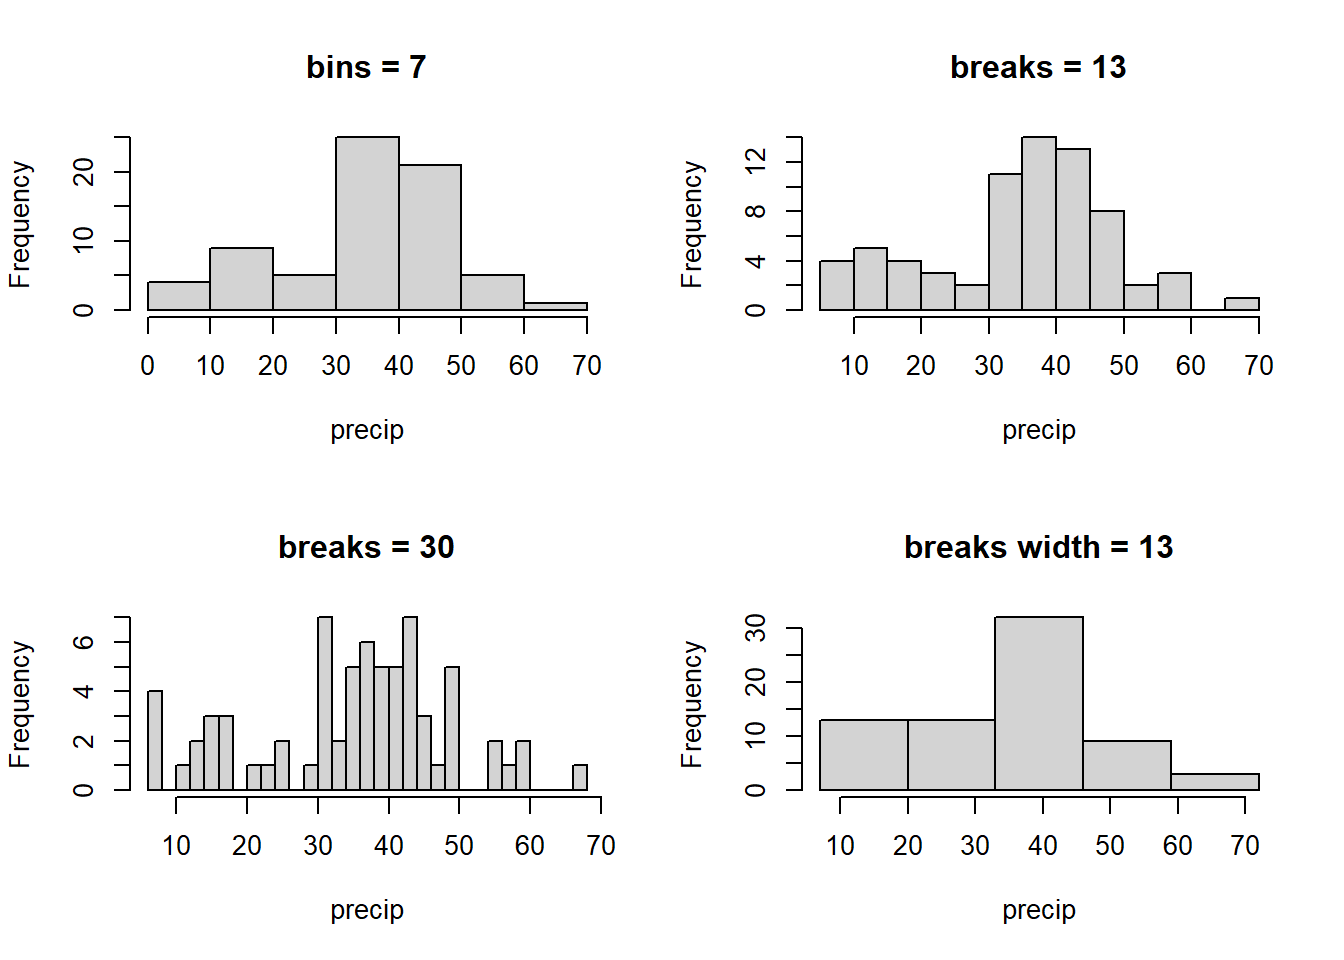
\includegraphics{Lab4_files/figure-latex/unnamed-chunk-5-1.pdf}

\hypertarget{section-9}{%
\subsection{10)}\label{section-9}}

These variables have low correlation so, we couldn't say that there is a
strong relation.

\begin{Shaded}
\begin{Highlighting}[]
\FunctionTok{cor}\NormalTok{(Galton}\SpecialCharTok{$}\NormalTok{height, Galton}\SpecialCharTok{$}\NormalTok{father)}
\end{Highlighting}
\end{Shaded}

\begin{verbatim}
## [1] 0.2753548
\end{verbatim}

\hypertarget{section-10}{%
\subsection{11)}\label{section-10}}

It's showing that how much height of father impacts on child height.

\begin{Shaded}
\begin{Highlighting}[]
\FunctionTok{lm}\NormalTok{(Galton}\SpecialCharTok{$}\NormalTok{height }\SpecialCharTok{\textasciitilde{}}\NormalTok{ Galton}\SpecialCharTok{$}\NormalTok{father, }\AttributeTok{data =}\NormalTok{ Galton)}
\end{Highlighting}
\end{Shaded}

\begin{verbatim}
## 
## Call:
## lm(formula = Galton$height ~ Galton$father, data = Galton)
## 
## Coefficients:
##   (Intercept)  Galton$father  
##       39.1104         0.3994
\end{verbatim}

\hypertarget{section-11}{%
\subsection{12)}\label{section-11}}

height = 0.3994 * father + 39.1104

Intercept is actually intercept of line equation.

\hypertarget{section-12}{%
\subsection{13)}\label{section-12}}

\begin{Shaded}
\begin{Highlighting}[]
\NormalTok{father }\OtherTok{\textless{}{-}} \FunctionTok{data.frame}\NormalTok{(}\AttributeTok{father =} \FunctionTok{c}\NormalTok{(}\DecValTok{70}\NormalTok{, }\DecValTok{75}\NormalTok{, }\DecValTok{80}\NormalTok{))}
\FunctionTok{predict}\NormalTok{(}\FunctionTok{lm}\NormalTok{(height }\SpecialCharTok{\textasciitilde{}}\NormalTok{ father, }\AttributeTok{data =}\NormalTok{ Galton), father)}
\end{Highlighting}
\end{Shaded}

\begin{verbatim}
##        1        2        3 
## 67.06708 69.06398 71.06089
\end{verbatim}

\hypertarget{section-13}{%
\subsection{14)}\label{section-13}}

\begin{Shaded}
\begin{Highlighting}[]
\FunctionTok{lm}\NormalTok{(height }\SpecialCharTok{\textasciitilde{}}\NormalTok{ father }\SpecialCharTok{+}\NormalTok{ mother, }\AttributeTok{data =}\NormalTok{ Galton)}
\end{Highlighting}
\end{Shaded}

\begin{verbatim}
## 
## Call:
## lm(formula = height ~ father + mother, data = Galton)
## 
## Coefficients:
## (Intercept)       father       mother  
##     22.3097       0.3799       0.2832
\end{verbatim}

\begin{Shaded}
\begin{Highlighting}[]
\NormalTok{Galton}
\end{Highlighting}
\end{Shaded}

\begin{verbatim}
##     family father mother sex height nkids
## 1        1   78.5   67.0   M   73.2     4
## 2        1   78.5   67.0   F   69.2     4
## 3        1   78.5   67.0   F   69.0     4
## 4        1   78.5   67.0   F   69.0     4
## 5        2   75.5   66.5   M   73.5     4
## 6        2   75.5   66.5   M   72.5     4
## 7        2   75.5   66.5   F   65.5     4
## 8        2   75.5   66.5   F   65.5     4
## 9        3   75.0   64.0   M   71.0     2
## 10       3   75.0   64.0   F   68.0     2
## 11       4   75.0   64.0   M   70.5     5
## 12       4   75.0   64.0   M   68.5     5
## 13       4   75.0   64.0   F   67.0     5
## 14       4   75.0   64.0   F   64.5     5
## 15       4   75.0   64.0   F   63.0     5
## 16       5   75.0   58.5   M   72.0     6
## 17       5   75.0   58.5   M   69.0     6
## 18       5   75.0   58.5   M   68.0     6
## 19       5   75.0   58.5   F   66.5     6
## 20       5   75.0   58.5   F   62.5     6
## 21       5   75.0   58.5   F   62.5     6
## 22       6   74.0   68.0   F   69.5     1
## 23       7   74.0   68.0   M   76.5     6
## 24       7   74.0   68.0   M   74.0     6
## 25       7   74.0   68.0   M   73.0     6
## 26       7   74.0   68.0   M   73.0     6
## 27       7   74.0   68.0   F   70.5     6
## 28       7   74.0   68.0   F   64.0     6
## 29       8   74.0   66.5   F   70.5     3
## 30       8   74.0   66.5   F   68.0     3
## 31       8   74.0   66.5   F   66.0     3
## 32       9   74.5   66.0   F   66.0     1
## 33      10   74.0   65.5   F   65.5     1
## 34      11   74.0   62.0   M   74.0     8
## 35      11   74.0   62.0   M   70.0     8
## 36      11   74.0   62.0   F   68.0     8
## 37      11   74.0   62.0   F   67.0     8
## 38      11   74.0   62.0   F   67.0     8
## 39      11   74.0   62.0   F   66.0     8
## 40      11   74.0   62.0   F   63.5     8
## 41      11   74.0   62.0   F   63.0     8
## 42      12   74.0   61.0   F   65.0     1
## 43      14   73.0   67.0   M   68.0     2
## 44      14   73.0   67.0   M   67.0     2
## 45      15   73.0   66.5   M   71.0     3
## 46      15   73.0   66.5   M   70.5     3
## 47      15   73.0   66.5   F   66.7     3
## 48      16   73.0   65.0   M   72.0     9
## 49      16   73.0   65.0   M   70.5     9
## 50      16   73.0   65.0   M   70.2     9
## 51      16   73.0   65.0   M   70.2     9
## 52      16   73.0   65.0   M   69.2     9
## 53      16   73.0   65.0   F   68.7     9
## 54      16   73.0   65.0   F   66.5     9
## 55      16   73.0   65.0   F   64.5     9
## 56      16   73.0   65.0   F   63.5     9
## 57      17   73.0   64.5   M   74.0     6
## 58      17   73.0   64.5   M   73.0     6
## 59      17   73.0   64.5   M   71.5     6
## 60      17   73.0   64.5   M   62.5     6
## 61      17   73.0   64.5   F   66.5     6
## 62      17   73.0   64.5   F   62.3     6
## 63      18   73.0   64.0   F   66.0     3
## 64      18   73.0   64.0   F   64.5     3
## 65      18   73.0   64.0   F   64.0     3
## 66      19   73.2   63.0   F   62.7     1
## 67      20   72.7   69.0   M   73.2     8
## 68      20   72.7   69.0   M   73.0     8
## 69      20   72.7   69.0   M   72.7     8
## 70      20   72.7   69.0   F   70.0     8
## 71      20   72.7   69.0   F   69.0     8
## 72      20   72.7   69.0   F   68.5     8
## 73      20   72.7   69.0   F   68.0     8
## 74      20   72.7   69.0   F   66.0     8
## 75      21   72.0   68.0   M   73.0     3
## 76      21   72.0   68.0   F   68.5     3
## 77      21   72.0   68.0   F   68.0     3
## 78      22   72.0   67.0   M   73.0     3
## 79      22   72.0   67.0   M   71.0     3
## 80      22   72.0   67.0   F   67.0     3
## 81      23   72.0   65.0   M   74.2     7
## 82      23   72.0   65.0   M   70.5     7
## 83      23   72.0   65.0   M   69.5     7
## 84      23   72.0   65.0   F   66.0     7
## 85      23   72.0   65.0   F   65.5     7
## 86      23   72.0   65.0   F   65.0     7
## 87      23   72.0   65.0   F   65.0     7
## 88      24   72.0   65.5   F   65.5     1
## 89      25   72.0   64.0   F   66.0     2
## 90      25   72.0   64.0   F   63.0     2
## 91      26   72.0   63.0   M   70.5     5
## 92      26   72.0   63.0   M   70.5     5
## 93      26   72.0   63.0   M   69.0     5
## 94      26   72.0   63.0   F   65.0     5
## 95      26   72.0   63.0   F   63.0     5
## 96      27   72.0   63.0   M   69.0     3
## 97      27   72.0   63.0   M   67.0     3
## 98      27   72.0   63.0   F   63.0     3
## 99      28   72.0   63.0   M   73.0     6
## 100     28   72.0   63.0   M   67.0     6
## 101     28   72.0   63.0   F   70.5     6
## 102     28   72.0   63.0   F   70.0     6
## 103     28   72.0   63.0   F   66.5     6
## 104     28   72.0   63.0   F   63.0     6
## 105     29   72.5   63.5   F   67.5     3
## 106     29   72.5   63.5   F   67.2     3
## 107     29   72.5   63.5   F   66.7     3
## 108     30   72.0   62.0   F   64.0     1
## 109     31   72.5   62.0   M   71.0     6
## 110     31   72.5   62.0   M   70.0     6
## 111     31   72.5   62.0   M   70.0     6
## 112     31   72.5   62.0   F   66.0     6
## 113     31   72.5   62.0   F   65.0     6
## 114     31   72.5   62.0   F   65.0     6
## 115     32   72.0   62.0   M   74.0     5
## 116     32   72.0   62.0   M   72.0     5
## 117     32   72.0   62.0   M   69.0     5
## 118     32   72.0   62.0   F   67.5     5
## 119     32   72.0   62.0   F   63.5     5
## 120     33   72.0   62.0   M   72.0     5
## 121     33   72.0   62.0   M   71.5     5
## 122     33   72.0   62.0   M   71.5     5
## 123     33   72.0   62.0   M   70.0     5
## 124     33   72.0   62.0   F   68.0     5
## 125     34   72.0   61.0   F   65.7     1
## 126     35   71.0   69.0   M   78.0     5
## 127     35   71.0   69.0   M   74.0     5
## 128     35   71.0   69.0   M   73.0     5
## 129     35   71.0   69.0   M   72.0     5
## 130     35   71.0   69.0   F   67.0     5
## 131     36   71.0   67.0   M   73.2     4
## 132     36   71.0   67.0   M   73.0     4
## 133     36   71.0   67.0   M   69.0     4
## 134     36   71.0   67.0   F   67.0     4
## 135     37   71.0   66.0   M   70.0     4
## 136     37   71.0   66.0   F   67.0     4
## 137     37   71.0   66.0   F   67.0     4
## 138     37   71.0   66.0   F   66.5     4
## 139     38   71.0   66.0   M   70.0     6
## 140     38   71.0   66.0   M   69.0     6
## 141     38   71.0   66.0   M   68.5     6
## 142     38   71.0   66.0   F   66.0     6
## 143     38   71.0   66.0   F   64.5     6
## 144     38   71.0   66.0   F   63.0     6
## 145     39   71.0   66.0   M   71.0     2
## 146     39   71.0   66.0   F   67.0     2
## 147     40   71.0   66.0   M   76.0     5
## 148     40   71.0   66.0   M   72.0     5
## 149     40   71.0   66.0   M   71.0     5
## 150     40   71.0   66.0   M   66.0     5
## 151     40   71.0   66.0   F   66.0     5
## 152     41   71.7   65.5   M   70.5     1
## 153     42   71.0   65.5   M   72.0     6
## 154     42   71.0   65.5   M   72.0     6
## 155     42   71.0   65.5   M   71.0     6
## 156     42   71.0   65.5   M   69.0     6
## 157     42   71.0   65.5   F   66.0     6
## 158     42   71.0   65.5   F   65.0     6
## 159     43   71.5   65.5   M   73.0     2
## 160     43   71.5   65.5   F   65.2     2
## 161     44   71.5   65.0   M   68.5     2
## 162     44   71.5   65.0   M   67.7     2
## 163     45   71.0   65.0   M   68.0     3
## 164     45   71.0   65.0   M   68.0     3
## 165     45   71.0   65.0   F   62.0     3
## 166     46   71.0   64.0   F   68.0     8
## 167     46   71.0   64.0   F   68.0     8
## 168     46   71.0   64.0   F   67.5     8
## 169     46   71.0   64.0   F   66.5     8
## 170     46   71.0   64.0   F   66.5     8
## 171     46   71.0   64.0   F   66.0     8
## 172     46   71.0   64.0   F   65.5     8
## 173     46   71.0   64.0   F   65.0     8
## 174     47   71.7   64.5   M   72.0     4
## 175     47   71.7   64.5   M   71.0     4
## 176     47   71.7   64.5   M   70.5     4
## 177     47   71.7   64.5   F   67.0     4
## 178     48   71.0   64.0   M   68.0     3
## 179     48   71.0   64.0   M   68.0     3
## 180     48   71.0   64.0   M   68.0     3
## 181     49   71.5   64.5   M   72.0     7
## 182     49   71.5   64.5   M   71.0     7
## 183     49   71.5   64.5   M   70.0     7
## 184     49   71.5   64.5   F   66.0     7
## 185     49   71.5   64.5   F   64.5     7
## 186     49   71.5   64.5   F   64.5     7
## 187     49   71.5   64.5   F   62.0     7
## 188     51   71.2   63.0   F   67.5     2
## 189     51   71.2   63.0   F   64.5     2
## 190     52   71.0   63.5   M   71.0     5
## 191     52   71.0   63.5   M   67.0     5
## 192     52   71.0   63.5   F   66.0     5
## 193     52   71.0   63.5   F   65.0     5
## 194     52   71.0   63.5   F   63.5     5
## 195     53   71.0   63.0   M   71.0     9
## 196     53   71.0   63.0   M   70.0     9
## 197     53   71.0   63.0   M   70.0     9
## 198     53   71.0   63.0   M   64.0     9
## 199     53   71.0   63.0   F   65.0     9
## 200     53   71.0   63.0   F   65.0     9
## 201     53   71.0   63.0   F   64.0     9
## 202     53   71.0   63.0   F   63.0     9
## 203     53   71.0   63.0   F   63.0     9
## 204     54   71.0   63.0   M   71.0     4
## 205     54   71.0   63.0   M   71.0     4
## 206     54   71.0   63.0   M   70.0     4
## 207     54   71.0   63.0   F   63.5     4
## 208     55   71.0   62.0   M   71.0     5
## 209     55   71.0   62.0   M   70.0     5
## 210     55   71.0   62.0   F   64.5     5
## 211     55   71.0   62.0   F   62.5     5
## 212     55   71.0   62.0   F   61.5     5
## 213     56   71.0   62.0   M   72.0     5
## 214     56   71.0   62.0   M   70.5     5
## 215     56   71.0   62.0   M   70.5     5
## 216     56   71.0   62.0   F   64.5     5
## 217     56   71.0   62.0   F   60.0     5
## 218     57   71.0   62.5   M   70.0     5
## 219     57   71.0   62.5   F   64.0     5
## 220     57   71.0   62.5   F   64.0     5
## 221     57   71.0   62.5   F   64.0     5
## 222     57   71.0   62.5   F   62.5     5
## 223     58   71.0   62.0   M   70.5     7
## 224     58   71.0   62.0   M   70.0     7
## 225     58   71.0   62.0   M   69.0     7
## 226     58   71.0   62.0   M   69.0     7
## 227     58   71.0   62.0   M   66.0     7
## 228     58   71.0   62.0   F   64.5     7
## 229     58   71.0   62.0   F   64.0     7
## 230     59   71.0   61.0   F   62.0     1
## 231     60   71.0   58.0   M   71.5     2
## 232     60   71.0   58.0   M   69.0     2
## 233     61   70.0   69.0   M   71.0     4
## 234     61   70.0   69.0   M   70.0     4
## 235     61   70.0   69.0   M   69.0     4
## 236     61   70.0   69.0   F   69.0     4
## 237     62   70.0   69.0   M   70.0     6
## 238     62   70.0   69.0   M   68.7     6
## 239     62   70.0   69.0   F   68.0     6
## 240     62   70.0   69.0   F   66.0     6
## 241     62   70.0   69.0   F   64.0     6
## 242     62   70.0   69.0   F   62.0     6
## 243     63   70.0   68.0   M   75.0     1
## 244     64   70.0   67.0   M   70.0     5
## 245     64   70.0   67.0   M   69.0     5
## 246     64   70.0   67.0   F   66.0     5
## 247     64   70.0   67.0   F   64.0     5
## 248     64   70.0   67.0   F   60.0     5
## 249     65   70.0   67.0   F   67.5     1
## 250     66   70.0   66.5   M   73.0    11
## 251     66   70.0   66.5   M   72.0    11
## 252     66   70.0   66.5   M   72.0    11
## 253     66   70.0   66.5   M   66.5    11
## 254     66   70.0   66.5   F   69.2    11
## 255     66   70.0   66.5   F   67.2    11
## 256     66   70.0   66.5   F   66.5    11
## 257     66   70.0   66.5   F   66.0    11
## 258     66   70.0   66.5   F   66.0    11
## 259     66   70.0   66.5   F   64.2    11
## 260     66   70.0   66.5   F   63.7    11
## 261     67   70.5   65.0   M   72.0     4
## 262     67   70.5   65.0   M   70.2     4
## 263     67   70.5   65.0   M   69.0     4
## 264     67   70.5   65.0   M   68.5     4
## 265     68   70.5   65.0   F   68.0     5
## 266     68   70.5   65.0   F   65.0     5
## 267     68   70.5   65.0   F   61.5     5
## 268     68   70.5   65.0   F   61.0     5
## 269     68   70.5   65.0   F   61.0     5
## 270     69   70.0   65.0   M   73.0     8
## 271     69   70.0   65.0   M   72.0     8
## 272     69   70.0   65.0   M   70.5     8
## 273     69   70.0   65.0   M   65.0     8
## 274     69   70.0   65.0   M   65.0     8
## 275     69   70.0   65.0   F   64.5     8
## 276     69   70.0   65.0   F   63.0     8
## 277     69   70.0   65.0   F   62.0     8
## 278     70   70.0   65.0   M   67.0     5
## 279     70   70.0   65.0   M   65.0     5
## 280     70   70.0   65.0   F   64.5     5
## 281     70   70.0   65.0   F   62.5     5
## 282     70   70.0   65.0   F   62.5     5
## 283     71   70.0   65.0   M   70.0     6
## 284     71   70.0   65.0   M   70.0     6
## 285     71   70.0   65.0   F   67.0     6
## 286     71   70.0   65.0   F   65.0     6
## 287     71   70.0   65.0   F   65.0     6
## 288     71   70.0   65.0   F   63.0     6
## 289     72   70.0   65.0   M   79.0     7
## 290     72   70.0   65.0   M   75.0     7
## 291     72   70.0   65.0   M   71.0     7
## 292     72   70.0   65.0   F   69.0     7
## 293     72   70.0   65.0   F   67.0     7
## 294     72   70.0   65.0   F   65.7     7
## 295     72   70.0   65.0   F   62.0     7
## 296     73   70.0   65.0   M   73.0     3
## 297     73   70.0   65.0   M   72.5     3
## 298     73   70.0   65.0   F   65.0     3
## 299     74   70.0   65.0   M   69.0     2
## 300     74   70.0   65.0   M   69.0     2
## 301     75   70.0   64.7   M   72.0     7
## 302     75   70.0   64.7   M   70.0     7
## 303     75   70.0   64.7   M   68.7     7
## 304     75   70.0   64.7   F   66.5     7
## 305     75   70.0   64.7   F   65.5     7
## 306     75   70.0   64.7   F   64.7     7
## 307     75   70.0   64.7   F   64.5     7
## 308     76   70.0   64.0   M   70.7     7
## 309     76   70.0   64.0   M   70.0     7
## 310     76   70.0   64.0   M   68.0     7
## 311     76   70.0   64.0   M   67.0     7
## 312     76   70.0   64.0   M   66.0     7
## 313     76   70.0   64.0   M   65.0     7
## 314     76   70.0   64.0   F   67.0     7
## 315     77   70.0   64.0   M   70.0     4
## 316     77   70.0   64.0   M   68.0     4
## 317     77   70.0   64.0   M   66.7     4
## 318     77   70.0   64.0   F   65.5     4
## 319     78   70.0   64.2   M   72.0     5
## 320     78   70.0   64.2   M   70.0     5
## 321     78   70.0   64.2   F   62.5     5
## 322     78   70.0   64.2   F   61.2     5
## 323     78   70.0   64.2   F   60.1     5
## 324     79   70.5   64.0   M   74.0     8
## 325     79   70.5   64.0   M   69.5     8
## 326     79   70.5   64.0   M   69.0     8
## 327     79   70.5   64.0   M   68.0     8
## 328     79   70.5   64.0   M   68.0     8
## 329     79   70.5   64.0   M   68.0     8
## 330     79   70.5   64.0   F   65.5     8
## 331     79   70.5   64.0   F   65.0     8
## 332     80   70.5   64.5   F   60.0     1
## 333     81   70.0   64.0   M   68.0     4
## 334     81   70.0   64.0   F   65.0     4
## 335     81   70.0   64.0   F   64.0     4
## 336     81   70.0   64.0   F   62.0     4
## 337     82   70.0   64.0   M   71.0     9
## 338     82   70.0   64.0   M   70.0     9
## 339     82   70.0   64.0   M   70.0     9
## 340     82   70.0   64.0   M   70.0     9
## 341     82   70.0   64.0   M   69.5     9
## 342     82   70.0   64.0   M   68.5     9
## 343     82   70.0   64.0   F   69.0     9
## 344     82   70.0   64.0   F   65.0     9
## 345     82   70.0   64.0   F   64.0     9
## 346     83   70.0   63.7   M   70.0     8
## 347     83   70.0   63.7   M   67.0     8
## 348     83   70.0   63.7   M   65.5     8
## 349     83   70.0   63.7   F   63.7     8
## 350     83   70.0   63.7   F   63.2     8
## 351     83   70.0   63.7   F   62.5     8
## 352     83   70.0   63.7   F   62.2     8
## 353     83   70.0   63.7   F   61.0     8
## 354     85   70.5   63.0   M   72.5     5
## 355     85   70.5   63.0   M   69.0     5
## 356     85   70.5   63.0   M   67.0     5
## 357     85   70.5   63.0   F   64.5     5
## 358     85   70.5   63.0   F   64.0     5
## 359     86   70.0   63.5   M   71.0     4
## 360     86   70.0   63.5   M   67.5     4
## 361     86   70.0   63.5   F   67.5     4
## 362     86   70.0   63.5   F   63.5     4
## 363     87   70.0   63.0   M   68.0     4
## 364     87   70.0   63.0   M   67.0     4
## 365     87   70.0   63.0   F   63.7     4
## 366     87   70.0   63.0   F   62.0     4
## 367     88   70.0   63.0   M   70.0     4
## 368     88   70.0   63.0   M   66.5     4
## 369     88   70.0   63.0   F   62.0     4
## 370     88   70.0   63.0   F   61.0     4
## 371     89   70.5   62.0   M   72.0     8
## 372     89   70.5   62.0   M   70.0     8
## 373     89   70.5   62.0   M   69.5     8
## 374     89   70.5   62.0   M   69.5     8
## 375     89   70.5   62.0   M   68.0     8
## 376     89   70.5   62.0   F   65.0     8
## 377     89   70.5   62.0   F   64.0     8
## 378     89   70.5   62.0   F   63.0     8
## 379     90   70.3   62.7   M   70.7     7
## 380     90   70.3   62.7   M   69.7     7
## 381     90   70.3   62.7   M   69.2     7
## 382     90   70.3   62.7   M   65.2     7
## 383     90   70.3   62.7   F   64.0     7
## 384     90   70.3   62.7   F   63.5     7
## 385     90   70.3   62.7   F   63.2     7
## 386     91   70.5   62.0   M   72.0     3
## 387     91   70.5   62.0   M   72.0     3
## 388     91   70.5   62.0   F   60.0     3
## 389     92   70.0   61.0   M   71.2     2
## 390     92   70.0   61.0   M   67.0     2
## 391     93   70.0   60.0   M   67.0     4
## 392     93   70.0   60.0   M   64.5     4
## 393     93   70.0   60.0   F   65.0     4
## 394     93   70.0   60.0   F   63.0     4
## 395     94   70.0   60.0   F   65.0     2
## 396     94   70.0   60.0   F   65.0     2
## 397     95   70.0   58.5   M   71.5     3
## 398     95   70.0   58.5   M   64.5     3
## 399     95   70.0   58.5   F   63.0     3
## 400     96   70.0   58.0   M   72.0     5
## 401     96   70.0   58.0   M   66.0     5
## 402     96   70.0   58.0   F   66.0     5
## 403     96   70.0   58.0   F   65.0     5
## 404     96   70.0   58.0   F   63.0     5
## 405     97   69.0   68.5   M   75.0    10
## 406     97   69.0   68.5   M   71.0    10
## 407     97   69.0   68.5   M   70.0    10
## 408     97   69.0   68.5   F   66.0    10
## 409     97   69.0   68.5   F   66.0    10
## 410     97   69.0   68.5   F   65.5    10
## 411     97   69.0   68.5   F   65.0    10
## 412     97   69.0   68.5   F   65.0    10
## 413     97   69.0   68.5   F   64.0    10
## 414     97   69.0   68.5   F   64.0    10
## 415     98   69.0   67.0   F   64.0     1
## 416     99   69.0   66.0   M   73.0     8
## 417     99   69.0   66.0   M   72.0     8
## 418     99   69.0   66.0   M   71.7     8
## 419     99   69.0   66.0   M   71.5     8
## 420     99   69.0   66.0   F   65.5     8
## 421     99   69.0   66.0   F   65.0     8
## 422     99   69.0   66.0   F   62.7     8
## 423     99   69.0   66.0   F   62.5     8
## 424    100   69.0   66.0   M   71.2     3
## 425    100   69.0   66.0   M   71.0     3
## 426    100   69.0   66.0   M   70.0     3
## 427    101   69.0   66.7   M   75.0     6
## 428    101   69.0   66.7   M   74.0     6
## 429    101   69.0   66.7   M   72.0     6
## 430    101   69.0   66.7   M   68.5     6
## 431    101   69.0   66.7   M   67.0     6
## 432    101   69.0   66.7   M   66.0     6
## 433    102   69.0   66.0   M   70.0     6
## 434    102   69.0   66.0   M   68.5     6
## 435    102   69.0   66.0   M   68.0     6
## 436    102   69.0   66.0   F   65.0     6
## 437    102   69.0   66.0   F   63.0     6
## 438    102   69.0   66.0   F   62.5     6
## 439    103   69.0   66.5   M   73.0     5
## 440    103   69.0   66.5   M   71.0     5
## 441    103   69.0   66.5   M   70.5     5
## 442    103   69.0   66.5   M   70.5     5
## 443    103   69.0   66.5   F   61.0     5
## 444    104   69.5   66.5   M   70.5     4
## 445    104   69.5   66.5   M   67.5     4
## 446    104   69.5   66.5   F   64.5     4
## 447    104   69.5   66.5   F   64.0     4
## 448    105   69.0   66.5   M   71.0     6
## 449    105   69.0   66.5   F   68.5     6
## 450    105   69.0   66.5   F   67.5     6
## 451    105   69.0   66.5   F   66.0     6
## 452    105   69.0   66.5   F   63.0     6
## 453    105   69.0   66.5   F   63.0     6
## 454    106   69.5   66.0   M   71.0     7
## 455    106   69.5   66.0   M   71.0     7
## 456    106   69.5   66.0   M   70.5     7
## 457    106   69.5   66.0   M   70.5     7
## 458    106   69.5   66.0   F   66.5     7
## 459    106   69.5   66.0   F   65.5     7
## 460    106   69.5   66.0   F   64.5     7
## 461    107   69.0   66.0   M   73.0     9
## 462    107   69.0   66.0   M   72.0     9
## 463    107   69.0   66.0   M   69.0     9
## 464    107   69.0   66.0   M   69.0     9
## 465    107   69.0   66.0   F   66.5     9
## 466    107   69.0   66.0   F   65.5     9
## 467    107   69.0   66.0   F   65.5     9
## 468    107   69.0   66.0   F   65.0     9
## 469    107   69.0   66.0   F   64.0     9
## 470    108   69.0   65.0   M   70.0     7
## 471    108   69.0   65.0   M   68.5     7
## 472    108   69.0   65.0   M   67.0     7
## 473    108   69.0   65.0   F   65.0     7
## 474    108   69.0   65.0   F   64.0     7
## 475    108   69.0   65.0   F   63.5     7
## 476    108   69.0   65.0   F   61.0     7
## 477    109   69.5   64.5   M   69.7     7
## 478    109   69.5   64.5   M   68.0     7
## 479    109   69.5   64.5   M   60.0     7
## 480    109   69.5   64.5   F   65.2     7
## 481    109   69.5   64.5   F   64.5     7
## 482    109   69.5   64.5   F   63.7     7
## 483    109   69.5   64.5   F   60.0     7
## 484    110   69.2   64.0   M   71.7     4
## 485    110   69.2   64.0   M   66.5     4
## 486    110   69.2   64.0   F   65.0     4
## 487    110   69.2   64.0   F   63.5     4
## 488    112   69.0   63.0   M   69.0     3
## 489    112   69.0   63.0   F   67.5     3
## 490    112   69.0   63.0   F   63.5     3
## 491    113   69.0   63.0   M   72.0     1
## 492    114   69.0   63.0   M   73.0     6
## 493    114   69.0   63.0   M   70.0     6
## 494    114   69.0   63.0   M   70.0     6
## 495    114   69.0   63.0   M   64.0     6
## 496    114   69.0   63.0   F   66.0     6
## 497    114   69.0   63.0   F   62.0     6
## 498    115   69.0   63.5   M   70.5     7
## 499    115   69.0   63.5   M   67.0     7
## 500    115   69.0   63.5   M   66.0     7
## 501    115   69.0   63.5   F   65.0     7
## 502    115   69.0   63.5   F   63.0     7
## 503    115   69.0   63.5   F   62.0     7
## 504    115   69.0   63.5   F   61.0     7
## 505    116   69.0   63.5   M   70.5     3
## 506    116   69.0   63.5   F   63.7     3
## 507    116   69.0   63.5   F   63.0     3
## 508    117   69.7   62.0   F   62.5     1
## 509    118   69.5   62.0   M   73.0     3
## 510    118   69.5   62.0   M   72.0     3
## 511    118   69.5   62.0   M   69.0     3
## 512    119   69.0   62.0   M   73.0     5
## 513    119   69.0   62.0   M   71.0     5
## 514    119   69.0   62.0   M   71.0     5
## 515    119   69.0   62.0   M   69.0     5
## 516    119   69.0   62.0   F   63.0     5
## 517    121   69.0   62.5   M   71.0     8
## 518    121   69.0   62.5   M   70.0     8
## 519    121   69.0   62.5   M   70.0     8
## 520    121   69.0   62.5   M   69.0     8
## 521    121   69.0   62.5   F   63.5     8
## 522    121   69.0   62.5   F   62.5     8
## 523    121   69.0   62.5   F   62.5     8
## 524    121   69.0   62.5   F   62.0     8
## 525    122   69.0   62.0   M   72.0     4
## 526    122   69.0   62.0   M   68.0     4
## 527    122   69.0   62.0   F   66.0     4
## 528    122   69.0   62.0   F   66.0     4
## 529    123   69.5   61.0   M   70.0     5
## 530    123   69.5   61.0   M   69.5     5
## 531    123   69.5   61.0   M   69.0     5
## 532    123   69.5   61.0   F   63.0     5
## 533    123   69.5   61.0   F   62.0     5
## 534    124   69.0   61.0   M   68.0     9
## 535    124   69.0   61.0   M   68.0     9
## 536    124   69.0   61.0   M   67.5     9
## 537    124   69.0   61.0   M   64.0     9
## 538    124   69.0   61.0   M   63.0     9
## 539    124   69.0   61.0   M   63.0     9
## 540    124   69.0   61.0   F   63.5     9
## 541    124   69.0   61.0   F   62.0     9
## 542    124   69.0   61.0   F   62.0     9
## 543    125   69.0   60.0   M   70.5     3
## 544    125   69.0   60.0   F   68.0     3
## 545    125   69.0   60.0   F   62.5     3
## 546    126   69.0   60.0   M   69.0     4
## 547    126   69.0   60.0   M   66.0     4
## 548    126   69.0   60.0   F   61.7     4
## 549    126   69.0   60.0   F   60.5     4
## 550    127   69.0   60.5   M   69.5     1
## 551    128   68.7   70.5   M   71.0     2
## 552    128   68.7   70.5   F   61.7     2
## 553    129   68.5   67.0   M   73.0     3
## 554    129   68.5   67.0   M   71.0     3
## 555    129   68.5   67.0   F   67.0     3
## 556    130   68.5   66.5   M   70.0    11
## 557    130   68.5   66.5   M   69.0    11
## 558    130   68.5   66.5   M   69.0    11
## 559    130   68.5   66.5   M   68.7    11
## 560    130   68.5   66.5   M   68.5    11
## 561    130   68.5   66.5   M   68.5    11
## 562    130   68.5   66.5   M   68.0    11
## 563    130   68.5   66.5   M   68.0    11
## 564    130   68.5   66.5   M   68.0    11
## 565    130   68.5   66.5   F   63.2    11
## 566    131   68.0   65.0   M   67.5     2
## 567    131   68.0   65.0   M   66.0     2
## 568    132   68.0   65.5   M   66.0     2
## 569    132   68.0   65.5   F   64.0     2
## 570    133   68.0   65.5   M   71.7     7
## 571    133   68.0   65.5   M   71.5     7
## 572    133   68.0   65.5   M   70.7     7
## 573    133   68.0   65.5   M   65.5     7
## 574    133   68.0   65.5   F   66.5     7
## 575    133   68.0   65.5   F   65.2     7
## 576    133   68.0   65.5   F   61.5     7
## 577    134   68.0   65.0   M   72.0     4
## 578    134   68.0   65.0   M   72.0     4
## 579    134   68.0   65.0   F   68.0     4
## 580    134   68.0   65.0   F   66.0     4
## 581    135   68.5   65.0   M   69.2     8
## 582    135   68.5   65.0   M   68.0     8
## 583    135   68.5   65.0   M   66.0     8
## 584    135   68.5   65.0   M   66.0     8
## 585    135   68.5   65.0   F   62.0     8
## 586    135   68.5   65.0   F   61.5     8
## 587    135   68.5   65.0   F   61.0     8
## 588    135   68.5   65.0   F   60.0     8
## 589    136   68.0   64.0   M   71.0    10
## 590    136   68.0   64.0   M   68.0    10
## 591    136   68.0   64.0   M   68.0    10
## 592    136   68.0   64.0   M   67.0    10
## 593    136   68.0   64.0   F   65.0    10
## 594    136   68.0   64.0   F   64.0    10
## 595    136   68.0   64.0   F   63.0    10
## 596    136   68.0   64.0   F   63.0    10
## 597    136   68.0   64.0   F   62.0    10
## 598    136   68.0   64.0   F   61.0    10
## 599    137   68.0   64.0   M   66.0     4
## 600    137   68.0   64.0   M   63.0     4
## 601    137   68.0   64.0   F   65.5     4
## 602    137   68.0   64.0   F   62.0     4
## 603    138   68.0   64.0   M   71.2     5
## 604    138   68.0   64.0   M   71.2     5
## 605    138   68.0   64.0   M   69.0     5
## 606    138   68.0   64.0   M   68.5     5
## 607    138   68.0   64.0   F   62.5     5
## 608    139   68.0   64.5   F   62.0     1
## 609    140   68.0   64.0   M   69.0    10
## 610    140   68.0   64.0   M   67.0    10
## 611    140   68.0   64.0   M   66.0    10
## 612    140   68.0   64.0   F   66.0    10
## 613    140   68.0   64.0   F   66.0    10
## 614    140   68.0   64.0   F   65.0    10
## 615    140   68.0   64.0   F   65.0    10
## 616    140   68.0   64.0   F   65.0    10
## 617    140   68.0   64.0   F   64.0    10
## 618    140   68.0   64.0   F   63.0    10
## 619    141   68.0   63.0   M   70.5     8
## 620    141   68.0   63.0   M   70.0     8
## 621    141   68.0   63.0   M   68.0     8
## 622    141   68.0   63.0   M   66.0     8
## 623    141   68.0   63.0   M   66.0     8
## 624    141   68.0   63.0   F   66.0     8
## 625    141   68.0   63.0   F   62.0     8
## 626    141   68.0   63.0   F   61.5     8
## 627    142   68.5   63.5   M   73.5     4
## 628    142   68.5   63.5   M   70.0     4
## 629    142   68.5   63.5   M   69.5     4
## 630    142   68.5   63.5   F   65.5     4
## 631    143   68.0   63.0   M   67.0     1
## 632    144   68.0   63.0   M   70.0     4
## 633    144   68.0   63.0   M   68.0     4
## 634    144   68.0   63.0   F   64.5     4
## 635    144   68.0   63.0   F   64.0     4
## 636    145   68.0   63.0   M   71.0     8
## 637    145   68.0   63.0   M   68.0     8
## 638    145   68.0   63.0   M   66.0     8
## 639    145   68.0   63.0   M   65.5     8
## 640    145   68.0   63.0   M   65.0     8
## 641    145   68.0   63.0   F   63.0     8
## 642    145   68.0   63.0   F   62.0     8
## 643    145   68.0   63.0   F   62.0     8
## 644    146   68.0   63.0   M   67.0     6
## 645    146   68.0   63.0   M   67.0     6
## 646    146   68.0   63.0   M   66.0     6
## 647    146   68.0   63.0   F   64.0     6
## 648    146   68.0   63.0   F   63.5     6
## 649    146   68.0   63.0   F   61.0     6
## 650    147   68.5   63.5   M   68.2     1
## 651    148   68.0   63.0   M   70.0     1
## 652    149   68.2   63.5   M   70.0     5
## 653    149   68.2   63.5   M   69.0     5
## 654    149   68.2   63.5   M   67.0     5
## 655    149   68.2   63.5   M   65.5     5
## 656    149   68.2   63.5   F   64.5     5
## 657    150   68.0   62.5   M   68.5     1
## 658    151   68.7   62.0   M   67.7     2
## 659    151   68.7   62.0   F   61.7     2
## 660    152   68.0   62.5   M   66.5     1
## 661    153   68.0   61.0   M   68.5     5
## 662    153   68.0   61.0   M   68.0     5
## 663    153   68.0   61.0   M   64.0     5
## 664    153   68.0   61.0   F   63.5     5
## 665    153   68.0   61.0   F   63.0     5
## 666    154   68.0   60.2   M   66.7     1
## 667    155   68.0   60.0   M   64.0     7
## 668    155   68.0   60.0   F   61.0     7
## 669    155   68.0   60.0   F   61.0     7
## 670    155   68.0   60.0   F   60.0     7
## 671    155   68.0   60.0   F   60.0     7
## 672    155   68.0   60.0   F   60.0     7
## 673    155   68.0   60.0   F   56.0     7
## 674    156   68.0   60.0   M   67.5     4
## 675    156   68.0   60.0   M   67.0     4
## 676    156   68.0   60.0   M   66.5     4
## 677    156   68.0   60.0   F   60.0     4
## 678    157   68.5   59.0   M   69.0     1
## 679    158   68.0   59.0   M   68.0    10
## 680    158   68.0   59.0   M   65.0    10
## 681    158   68.0   59.0   M   64.7    10
## 682    158   68.0   59.0   M   64.0    10
## 683    158   68.0   59.0   M   64.0    10
## 684    158   68.0   59.0   M   63.0    10
## 685    158   68.0   59.0   F   65.0    10
## 686    158   68.0   59.0   F   65.0    10
## 687    158   68.0   59.0   F   62.0    10
## 688    158   68.0   59.0   F   61.0    10
## 689    159   67.0   66.2   M   72.7     5
## 690    159   67.0   66.2   M   72.7     5
## 691    159   67.0   66.2   M   71.5     5
## 692    159   67.0   66.2   F   65.5     5
## 693    159   67.0   66.2   F   63.5     5
## 694    160   67.0   66.5   M   71.0     1
## 695    162   67.0   65.0   M   69.7     6
## 696    162   67.0   65.0   M   67.5     6
## 697    162   67.0   65.0   F   65.5     6
## 698    162   67.0   65.0   F   65.0     6
## 699    162   67.0   65.0   F   64.5     6
## 700    162   67.0   65.0   F   63.5     6
## 701    163   67.0   65.5   M   70.0     5
## 702    163   67.0   65.5   M   69.0     5
## 703    163   67.0   65.5   F   65.5     5
## 704    163   67.0   65.5   F   65.5     5
## 705    163   67.0   65.5   F   63.0     5
## 706    164   67.0   65.5   M   70.0     4
## 707    164   67.0   65.5   M   67.7     4
## 708    164   67.0   65.5   F   63.0     4
## 709    164   67.0   65.5   F   60.0     4
## 710    165   67.0   65.0   M   65.0     3
## 711    165   67.0   65.0   F   62.0     3
## 712    165   67.0   65.0   F   62.0     3
## 713    166   67.5   65.0   M   71.0    11
## 714    166   67.5   65.0   M   69.0    11
## 715    166   67.5   65.0   F   64.0    11
## 716    166   67.5   65.0   F   64.0    11
## 717    166   67.5   65.0   F   63.0    11
## 718    166   67.5   65.0   F   63.0    11
## 719    166   67.5   65.0   F   63.0    11
## 720    166   67.5   65.0   F   63.0    11
## 721    166   67.5   65.0   F   63.0    11
## 722    166   67.5   65.0   F   62.5    11
## 723    166   67.5   65.0   F   62.0    11
## 724    167   67.0   64.0   M   71.5     4
## 725    167   67.0   64.0   M   70.0     4
## 726    167   67.0   64.0   M   67.0     4
## 727    167   67.0   64.0   M   67.0     4
## 728    168   67.0   63.5   M   71.0     8
## 729    168   67.0   63.5   M   70.2     8
## 730    168   67.0   63.5   M   69.2     8
## 731    168   67.0   63.5   M   68.5     8
## 732    168   67.0   63.5   M   68.0     8
## 733    168   67.0   63.5   M   67.0     8
## 734    168   67.0   63.5   M   65.5     8
## 735    168   67.0   63.5   F   63.5     8
## 736    169   67.0   63.0   M   69.0     3
## 737    169   67.0   63.0   M   68.0     3
## 738    169   67.0   63.0   F   63.0     3
## 739    170   67.5   62.0   M   70.0     5
## 740    170   67.5   62.0   M   69.5     5
## 741    170   67.5   62.0   M   69.0     5
## 742    170   67.5   62.0   M   68.5     5
## 743    170   67.5   62.0   F   66.0     5
## 744    171   67.0   61.0   M   67.0     1
## 745    172   66.0   67.0   M   70.5     8
## 746    172   66.0   67.0   M   70.5     8
## 747    172   66.0   67.0   M   67.0     8
## 748    172   66.0   67.0   M   66.0     8
## 749    172   66.0   67.0   M   66.0     8
## 750    172   66.0   67.0   F   62.0     8
## 751    172   66.0   67.0   F   62.0     8
## 752    172   66.0   67.0   F   61.5     8
## 753    173   66.0   67.0   M   72.0     9
## 754    173   66.0   67.0   M   65.0     9
## 755    173   66.0   67.0   M   65.0     9
## 756    173   66.0   67.0   F   67.0     9
## 757    173   66.0   67.0   F   64.0     9
## 758    173   66.0   67.0   F   64.0     9
## 759    173   66.0   67.0   F   62.0     9
## 760    173   66.0   67.0   F   60.0     9
## 761    173   66.0   67.0   F   60.0     9
## 762    174   66.0   66.0   M   66.0     5
## 763    174   66.0   66.0   M   65.0     5
## 764    174   66.0   66.0   F   67.0     5
## 765    174   66.0   66.0   F   66.5     5
## 766    174   66.0   66.0   F   65.5     5
## 767    175   66.0   66.0   M   72.0     6
## 768    175   66.0   66.0   M   68.0     6
## 769    175   66.0   66.0   F   66.0     6
## 770    175   66.0   66.0   F   65.0     6
## 771    175   66.0   66.0   F   62.0     6
## 772    175   66.0   66.0   F   61.0     6
## 773    176   66.5   65.0   M   68.7     8
## 774    176   66.5   65.0   M   68.5     8
## 775    176   66.5   65.0   M   66.5     8
## 776    176   66.5   65.0   M   64.5     8
## 777    176   66.5   65.0   F   62.5     8
## 778    176   66.5   65.0   F   60.5     8
## 779    176   66.5   65.0   F   60.5     8
## 780    176   66.5   65.0   F   57.5     8
## 781    177   66.0   65.5   M   72.0     5
## 782    177   66.0   65.5   M   71.0     5
## 783    177   66.0   65.5   M   67.0     5
## 784    177   66.0   65.5   F   66.0     5
## 785    177   66.0   65.5   F   65.0     5
## 786    178   66.0   63.0   M   70.0     1
## 787    179   66.0   63.5   F   64.5     2
## 788    179   66.0   63.5   F   62.0     2
## 789    180   66.5   63.0   M   67.2     6
## 790    180   66.5   63.0   M   67.0     6
## 791    180   66.5   63.0   M   65.0     6
## 792    180   66.5   63.0   F   65.0     6
## 793    180   66.5   63.0   F   65.0     6
## 794    180   66.5   63.0   F   63.0     6
## 795    181   66.5   62.5   M   70.0     7
## 796    181   66.5   62.5   M   68.0     7
## 797    181   66.5   62.5   F   63.5     7
## 798    181   66.5   62.5   F   62.5     7
## 799    181   66.5   62.5   F   62.5     7
## 800    181   66.5   62.5   F   62.5     7
## 801    181   66.5   62.5   F   62.5     7
## 802    182   66.0   61.5   M   70.0     1
## 803    183   66.0   60.0   M   68.0     4
## 804    183   66.0   60.0   M   67.0     4
## 805    183   66.0   60.0   M   65.0     4
## 806    183   66.0   60.0   F   60.0     4
## 807    184   66.0   60.0   M   65.0     1
## 808    185   66.0   59.0   M   68.0    15
## 809    185   66.0   59.0   M   67.0    15
## 810    185   66.0   59.0   M   66.5    15
## 811    185   66.0   59.0   M   66.0    15
## 812    185   66.0   59.0   M   65.7    15
## 813    185   66.0   59.0   M   65.5    15
## 814    185   66.0   59.0   M   65.0    15
## 815    185   66.0   59.0   F   65.0    15
## 816    185   66.0   59.0   F   64.0    15
## 817    185   66.0   59.0   F   63.0    15
## 818    185   66.0   59.0   F   62.0    15
## 819    185   66.0   59.0   F   61.0    15
## 820    185   66.0   59.0   F   60.0    15
## 821    185   66.0   59.0   F   58.0    15
## 822    185   66.0   59.0   F   57.0    15
## 823    186   65.0   67.0   M   66.5     4
## 824    186   65.0   67.0   M   66.0     4
## 825    186   65.0   67.0   M   66.0     4
## 826    186   65.0   67.0   F   65.0     4
## 827    187   65.0   67.0   F   63.0     1
## 828    188   65.0   66.0   M   63.0     4
## 829    188   65.0   66.0   F   63.0     4
## 830    188   65.0   66.0   F   63.0     4
## 831    188   65.0   66.0   F   60.0     4
## 832    190   65.0   65.0   M   69.0     9
## 833    190   65.0   65.0   M   68.0     9
## 834    190   65.0   65.0   M   68.0     9
## 835    190   65.0   65.0   F   65.0     9
## 836    190   65.0   65.0   F   65.0     9
## 837    190   65.0   65.0   F   62.0     9
## 838    190   65.0   65.0   F   62.0     9
## 839    190   65.0   65.0   F   61.0     9
## 840    190   65.0   65.0   F   59.0     9
## 841    191   65.0   65.5   M   70.7     2
## 842    191   65.0   65.5   F   65.5     2
## 843    192   65.0   65.0   M   69.2     6
## 844    192   65.0   65.0   M   69.0     6
## 845    192   65.0   65.0   M   68.0     6
## 846    192   65.0   65.0   M   67.7     6
## 847    192   65.0   65.0   F   64.5     6
## 848    192   65.0   65.0   F   60.5     6
## 849    193   65.0   64.0   M   67.0     6
## 850    193   65.0   64.0   M   67.0     6
## 851    193   65.0   64.0   F   64.0     6
## 852    193   65.0   64.0   F   64.0     6
## 853    193   65.0   64.0   F   62.5     6
## 854    193   65.0   64.0   F   60.5     6
## 855    194   65.0   63.0   M   70.0     2
## 856    194   65.0   63.0   F   63.0     2
## 857    195   65.0   63.0   M   66.0     3
## 858    195   65.0   63.0   M   66.0     3
## 859    195   65.0   63.0   F   63.0     3
## 860    196   65.5   63.0   M   71.0     4
## 861    196   65.5   63.0   M   71.0     4
## 862    196   65.5   63.0   M   69.0     4
## 863    196   65.5   63.0   F   63.5     4
## 864    197   65.5   60.0   M   68.0     5
## 865    197   65.5   60.0   M   68.0     5
## 866    197   65.5   60.0   M   67.0     5
## 867    197   65.5   60.0   M   67.0     5
## 868    197   65.5   60.0   F   62.0     5
## 869    198   64.0   64.0   M   71.5     7
## 870    198   64.0   64.0   M   68.0     7
## 871    198   64.0   64.0   F   65.5     7
## 872    198   64.0   64.0   F   64.0     7
## 873    198   64.0   64.0   F   62.0     7
## 874    198   64.0   64.0   F   62.0     7
## 875    198   64.0   64.0   F   61.0     7
## 876    199   64.0   64.0   M   70.5     7
## 877    199   64.0   64.0   M   68.0     7
## 878    199   64.0   64.0   F   67.0     7
## 879    199   64.0   64.0   F   65.0     7
## 880    199   64.0   64.0   F   64.0     7
## 881    199   64.0   64.0   F   64.0     7
## 882    199   64.0   64.0   F   60.0     7
## 883    200   64.0   63.0   M   64.5     1
## 884    201   64.0   60.0   M   66.0     2
## 885    201   64.0   60.0   F   60.0     2
## 886    203   62.0   66.0   M   64.0     3
## 887    203   62.0   66.0   F   62.0     3
## 888    203   62.0   66.0   F   61.0     3
## 889    204   62.5   63.0   M   66.5     2
## 890    204   62.5   63.0   F   57.0     2
## 891   136A   68.5   65.0   M   72.0     8
## 892   136A   68.5   65.0   M   70.5     8
## 893   136A   68.5   65.0   M   68.7     8
## 894   136A   68.5   65.0   M   68.5     8
## 895   136A   68.5   65.0   M   67.7     8
## 896   136A   68.5   65.0   F   64.0     8
## 897   136A   68.5   65.0   F   63.5     8
## 898   136A   68.5   65.0   F   63.0     8
\end{verbatim}

\hypertarget{section-14}{%
\subsection{15)}\label{section-14}}

normal distribution of residuals

\begin{Shaded}
\begin{Highlighting}[]
\NormalTok{mlr }\OtherTok{\textless{}{-}} \FunctionTok{lm}\NormalTok{(height }\SpecialCharTok{\textasciitilde{}}\NormalTok{ father }\SpecialCharTok{+}\NormalTok{ mother, }\AttributeTok{data =}\NormalTok{ Galton)}
\NormalTok{residuals }\OtherTok{=}\NormalTok{ Galton}\SpecialCharTok{$}\NormalTok{height }\SpecialCharTok{{-}} \FunctionTok{predict}\NormalTok{(mlr, Galton)}
\FunctionTok{hist}\NormalTok{(residuals)}
\end{Highlighting}
\end{Shaded}

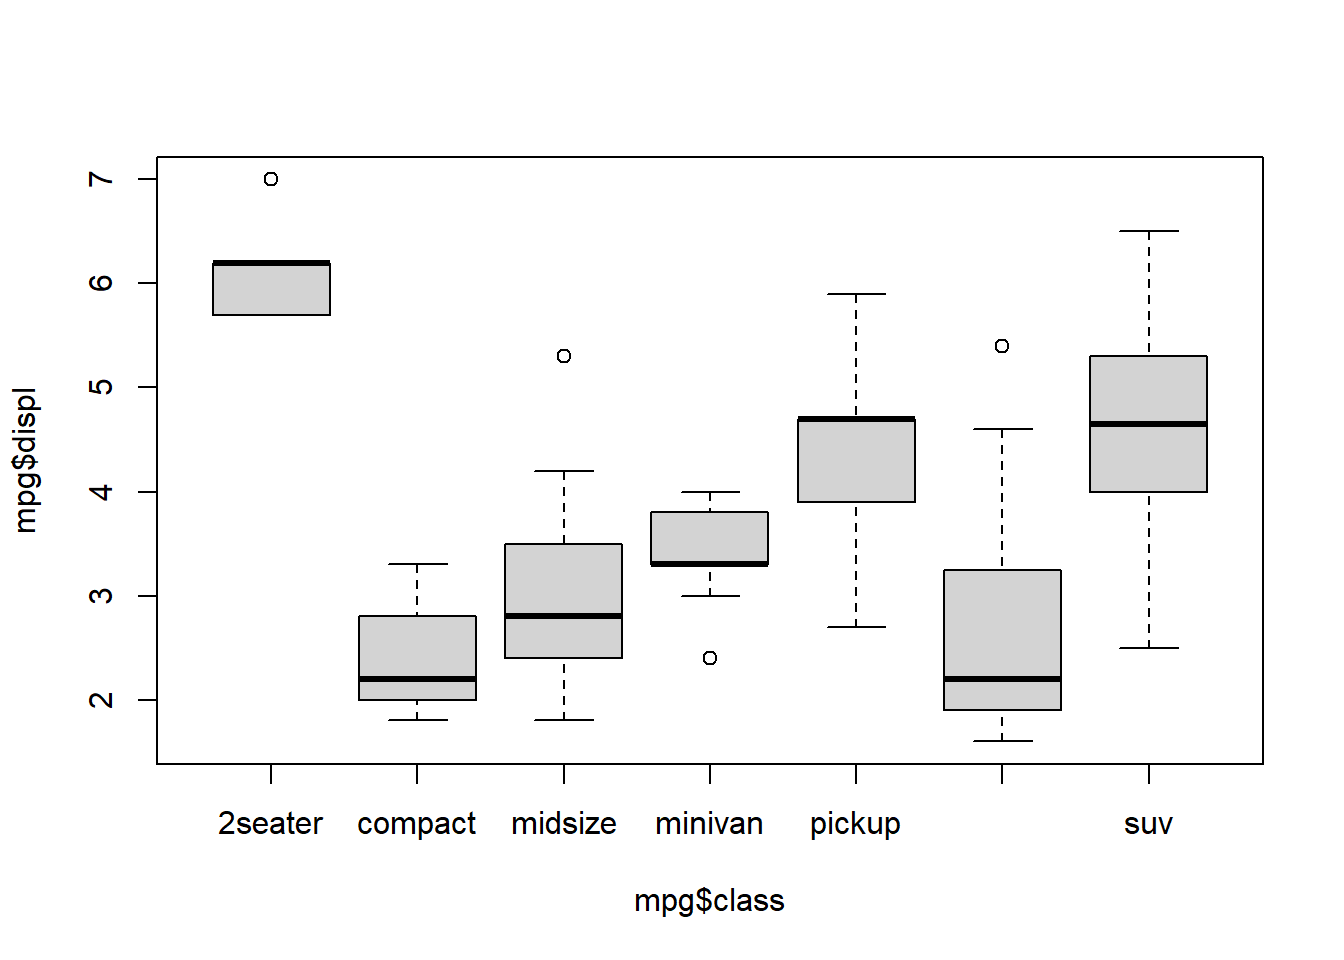
\includegraphics{Lab4_files/figure-latex/unnamed-chunk-10-1.pdf}

\hypertarget{section-15}{%
\subsection{16)}\label{section-15}}

normal distribution of resudals

\begin{Shaded}
\begin{Highlighting}[]
\FunctionTok{qqplot}\NormalTok{(residuals, }\FunctionTok{rnorm}\NormalTok{(}\FunctionTok{length}\NormalTok{(residuals)))}
\end{Highlighting}
\end{Shaded}

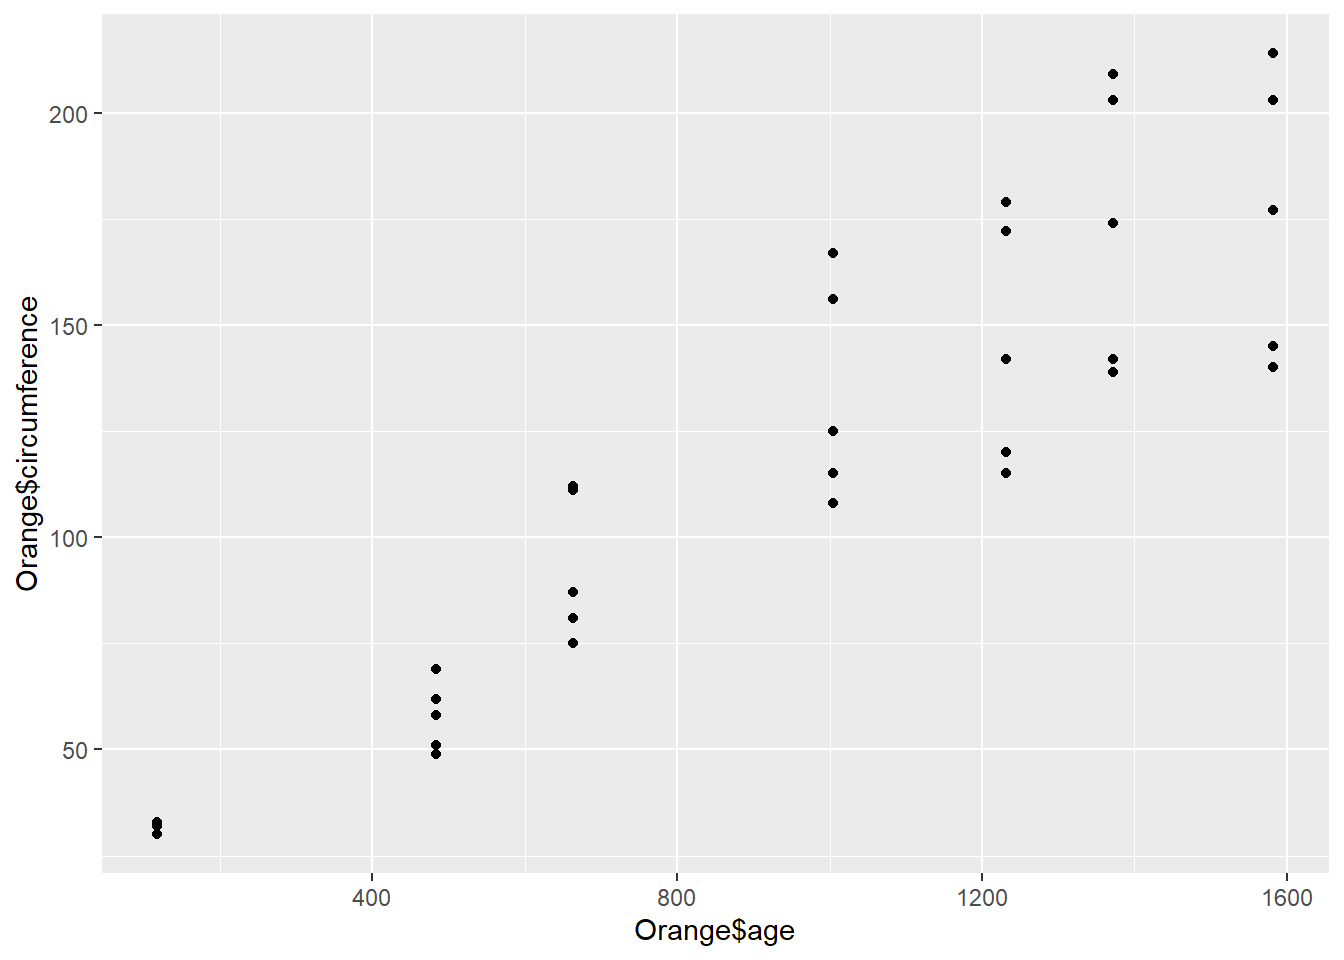
\includegraphics{Lab4_files/figure-latex/unnamed-chunk-11-1.pdf}

\hypertarget{section-16}{%
\subsection{17)}\label{section-16}}

Linearity

\begin{Shaded}
\begin{Highlighting}[]
\FunctionTok{plot}\NormalTok{(residuals, Galton}\SpecialCharTok{$}\NormalTok{father)}
\end{Highlighting}
\end{Shaded}

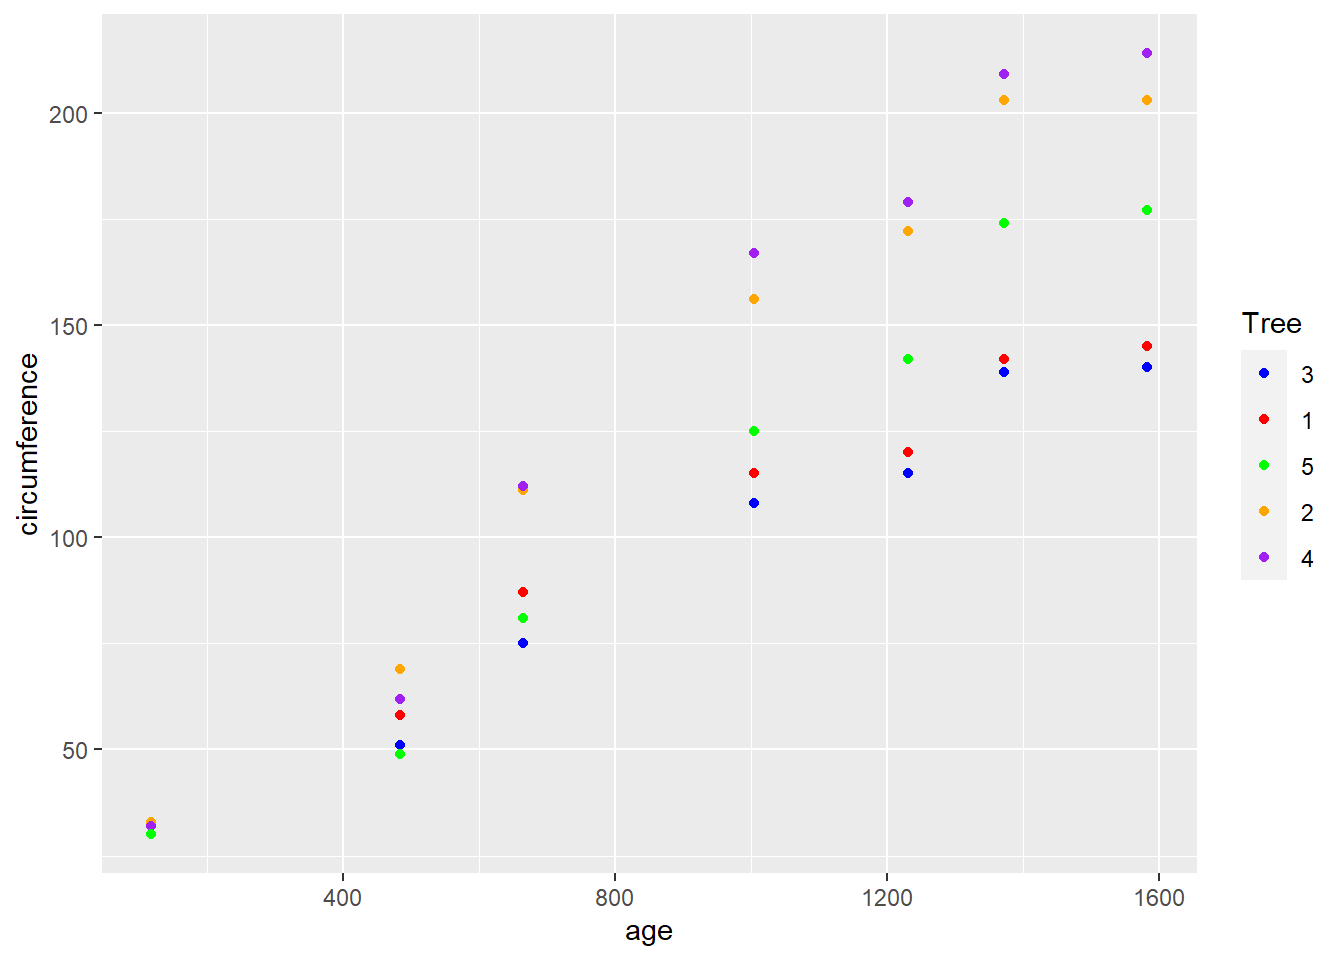
\includegraphics{Lab4_files/figure-latex/unnamed-chunk-12-1.pdf}

\begin{Shaded}
\begin{Highlighting}[]
\FunctionTok{plot}\NormalTok{(residuals, Galton}\SpecialCharTok{$}\NormalTok{mother)}
\end{Highlighting}
\end{Shaded}

\includegraphics{Lab4_files/figure-latex/unnamed-chunk-12-2.pdf}

\hypertarget{section-17}{%
\subsection{18)}\label{section-17}}

constant variablity

\begin{Shaded}
\begin{Highlighting}[]
\FunctionTok{plot}\NormalTok{(residuals)}
\end{Highlighting}
\end{Shaded}

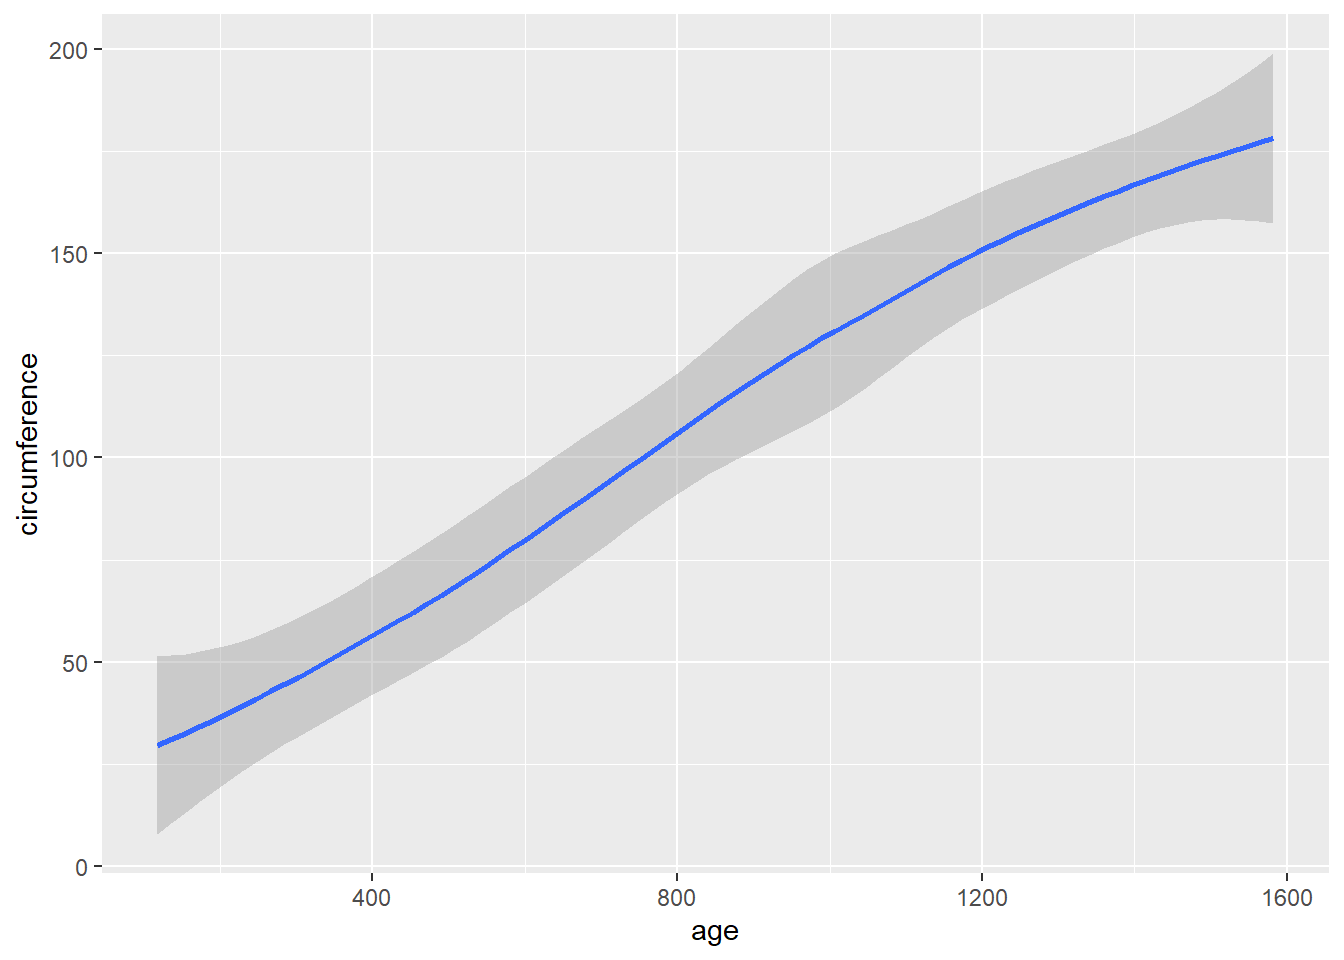
\includegraphics{Lab4_files/figure-latex/unnamed-chunk-13-1.pdf}

\hypertarget{section-18}{%
\subsection{19 \& 20)}\label{section-18}}

It is statistically significant

\begin{Shaded}
\begin{Highlighting}[]
\FunctionTok{lm}\NormalTok{(height }\SpecialCharTok{\textasciitilde{}}\NormalTok{ father }\SpecialCharTok{+}\NormalTok{ mother }\SpecialCharTok{+}\NormalTok{ sex, }\AttributeTok{data =}\NormalTok{ Galton)}
\end{Highlighting}
\end{Shaded}

\begin{verbatim}
## 
## Call:
## lm(formula = height ~ father + mother + sex, data = Galton)
## 
## Coefficients:
## (Intercept)       father       mother         sexM  
##     15.3448       0.4060       0.3215       5.2260
\end{verbatim}

\hypertarget{section-19}{%
\subsection{21)}\label{section-19}}

By this method, we can just remove nkids.

As you can see residuals distribution is almost normal and they have
constant variability.

relation between response variable and explanatory variables are linear.

\begin{Shaded}
\begin{Highlighting}[]
\NormalTok{lmr }\OtherTok{=} \FunctionTok{lm}\NormalTok{(height }\SpecialCharTok{\textasciitilde{}}\NormalTok{father }\SpecialCharTok{+}\NormalTok{ mother }\SpecialCharTok{+}\NormalTok{ sex, }\AttributeTok{data =}\NormalTok{ Galton)}
\NormalTok{residuals }\OtherTok{=}\NormalTok{ Galton}\SpecialCharTok{$}\NormalTok{height }\SpecialCharTok{{-}} \FunctionTok{predict}\NormalTok{(lmr, Galton)}
\FunctionTok{hist}\NormalTok{(residuals)}
\end{Highlighting}
\end{Shaded}

\includegraphics{Lab4_files/figure-latex/unnamed-chunk-15-1.pdf}

\begin{Shaded}
\begin{Highlighting}[]
\FunctionTok{plot}\NormalTok{(residuals)}
\end{Highlighting}
\end{Shaded}

\includegraphics{Lab4_files/figure-latex/unnamed-chunk-15-2.pdf}

\hypertarget{d-logistic-regression}{%
\section{d) Logistic Regression}\label{d-logistic-regression}}

\hypertarget{section-20}{%
\subsection{22)}\label{section-20}}

\begin{Shaded}
\begin{Highlighting}[]
\FunctionTok{library}\NormalTok{(tidyr)}
\FunctionTok{library}\NormalTok{(COUNT)}
\FunctionTok{data}\NormalTok{(}\StringTok{"titanic"}\NormalTok{)}
\NormalTok{titanic}\SpecialCharTok{$}\NormalTok{survived }\OtherTok{\textless{}{-}} \FunctionTok{ifelse}\NormalTok{(titanic}\SpecialCharTok{$}\NormalTok{survived }\SpecialCharTok{==} \StringTok{\textquotesingle{}yes\textquotesingle{}}\NormalTok{, T, F)}
\NormalTok{eq }\OtherTok{\textless{}{-}} \FunctionTok{glm}\NormalTok{(survived }\SpecialCharTok{\textasciitilde{}}\NormalTok{ ., }\AttributeTok{data =}\NormalTok{ titanic, }\AttributeTok{family =} \FunctionTok{binomial}\NormalTok{(}\AttributeTok{link =} \StringTok{\textquotesingle{}logit\textquotesingle{}}\NormalTok{))}
\FunctionTok{summary}\NormalTok{(eq)}
\end{Highlighting}
\end{Shaded}

\begin{verbatim}
## 
## Call:
## glm(formula = survived ~ ., family = binomial(link = "logit"), 
##     data = titanic)
## 
## Deviance Residuals: 
##     Min       1Q   Median       3Q      Max  
## -2.0652  -0.6718  -0.4740   0.7930   2.1175  
## 
## Coefficients:
##                Estimate Std. Error z value Pr(>|z|)    
## (Intercept)      3.0619     0.2980  10.275  < 2e-16 ***
## class2nd class  -1.0106     0.1949  -5.184 2.17e-07 ***
## class3rd class  -1.7664     0.1707 -10.347  < 2e-16 ***
## ageadults       -1.0556     0.2427  -4.350 1.36e-05 ***
## sexman          -2.3695     0.1453 -16.313  < 2e-16 ***
## ---
## Signif. codes:  0 '***' 0.001 '**' 0.01 '*' 0.05 '.' 0.1 ' ' 1
## 
## (Dispersion parameter for binomial family taken to be 1)
## 
##     Null deviance: 1746.8  on 1315  degrees of freedom
## Residual deviance: 1276.2  on 1311  degrees of freedom
## AIC: 1286.2
## 
## Number of Fisher Scoring iterations: 4
\end{verbatim}

\hypertarget{section-21}{%
\subsection{23)}\label{section-21}}

\begin{Shaded}
\begin{Highlighting}[]
\FunctionTok{head}\NormalTok{(titanic)}
\end{Highlighting}
\end{Shaded}

\begin{verbatim}
##       class    age sex survived
## 1 1st class adults man     TRUE
## 2 1st class adults man     TRUE
## 3 1st class adults man     TRUE
## 4 1st class adults man     TRUE
## 5 1st class adults man     TRUE
## 6 1st class adults man     TRUE
\end{verbatim}

\begin{Shaded}
\begin{Highlighting}[]
\NormalTok{smpl }\OtherTok{=} \FunctionTok{data.frame}\NormalTok{(}\AttributeTok{class =} \FunctionTok{c}\NormalTok{(}\StringTok{\textquotesingle{}2nd class\textquotesingle{}}\NormalTok{), }\AttributeTok{age =} \StringTok{\textquotesingle{}adults\textquotesingle{}}\NormalTok{, }\AttributeTok{sex =} \StringTok{\textquotesingle{}man\textquotesingle{}}\NormalTok{)}
\FunctionTok{predict}\NormalTok{(eq, smpl, }\AttributeTok{type =} \StringTok{\textquotesingle{}response\textquotesingle{}}\NormalTok{)}
\end{Highlighting}
\end{Shaded}

\begin{verbatim}
##         1 
## 0.2020148
\end{verbatim}

\hypertarget{section-22}{%
\subsection{24)}\label{section-22}}

\begin{Shaded}
\begin{Highlighting}[]
\NormalTok{titanic }\OtherTok{\textless{}{-}} \FunctionTok{droplevels}\NormalTok{(titanic)}
\NormalTok{smpl }\OtherTok{\textless{}{-}}\NormalTok{ titanic }\SpecialCharTok{\%\textgreater{}\%} \FunctionTok{expand}\NormalTok{(class, age, sex)}
\NormalTok{smpl}
\end{Highlighting}
\end{Shaded}

\begin{verbatim}
## # A tibble: 12 x 3
##    class     age    sex  
##    <fct>     <fct>  <fct>
##  1 1st class child  women
##  2 1st class child  man  
##  3 1st class adults women
##  4 1st class adults man  
##  5 2nd class child  women
##  6 2nd class child  man  
##  7 2nd class adults women
##  8 2nd class adults man  
##  9 3rd class child  women
## 10 3rd class child  man  
## 11 3rd class adults women
## 12 3rd class adults man
\end{verbatim}

\begin{Shaded}
\begin{Highlighting}[]
\NormalTok{smpl}\SpecialCharTok{$}\NormalTok{probabilty }\OtherTok{\textless{}{-}} \FunctionTok{predict}\NormalTok{(eq, smpl, }\AttributeTok{type =} \StringTok{\textquotesingle{}response\textquotesingle{}}\NormalTok{)}
\NormalTok{smpl}
\end{Highlighting}
\end{Shaded}

\begin{verbatim}
## # A tibble: 12 x 4
##    class     age    sex   probabilty
##    <fct>     <fct>  <fct>      <dbl>
##  1 1st class child  women      0.955
##  2 1st class child  man        0.667
##  3 1st class adults women      0.881
##  4 1st class adults man        0.410
##  5 2nd class child  women      0.886
##  6 2nd class child  man        0.421
##  7 2nd class adults women      0.730
##  8 2nd class adults man        0.202
##  9 3rd class child  women      0.785
## 10 3rd class child  man        0.255
## 11 3rd class adults women      0.560
## 12 3rd class adults man        0.106
\end{verbatim}

\hypertarget{section-23}{%
\subsection{25)}\label{section-23}}

\begin{Shaded}
\begin{Highlighting}[]
\NormalTok{titanic}\SpecialCharTok{$}\NormalTok{predicted\_survied }\OtherTok{\textless{}{-}} \FunctionTok{ifelse}\NormalTok{(}\FunctionTok{predict}\NormalTok{(eq, titanic, }\AttributeTok{type =} \StringTok{\textquotesingle{}response\textquotesingle{}}\NormalTok{) }\SpecialCharTok{\textgreater{}=} \FloatTok{0.5}\NormalTok{, T, F)}
\FunctionTok{sum}\NormalTok{(titanic}\SpecialCharTok{$}\NormalTok{survived }\SpecialCharTok{==}\NormalTok{ titanic}\SpecialCharTok{$}\NormalTok{predicted\_survied)}
\end{Highlighting}
\end{Shaded}

\begin{verbatim}
## [1] 1023
\end{verbatim}

\begin{Shaded}
\begin{Highlighting}[]
\FunctionTok{sum}\NormalTok{(titanic}\SpecialCharTok{$}\NormalTok{survived }\SpecialCharTok{==}\NormalTok{ titanic}\SpecialCharTok{$}\NormalTok{predicted\_survied) }\SpecialCharTok{/} \FunctionTok{length}\NormalTok{(titanic}\SpecialCharTok{$}\NormalTok{survived)}
\end{Highlighting}
\end{Shaded}

\begin{verbatim}
## [1] 0.7773556
\end{verbatim}

\hypertarget{section-24}{%
\subsection{26)}\label{section-24}}

No, it isn't valid, because there should be a lot of equipment to
prevent people from dying in the sea after the Titanic accident.

If these two accidents happened at the same time and with the same
available equipment, we could predict the number of survivors of second
accident by using first accident's data.

\end{document}
